\textit{	
Source: Julia Programming for Operations Research 2$^{nd}$ edition (Online).\\
Available at: http://www.chkwon.net/julia - published by Changhyun Kwon
}

Consider the following network where the combined supplies from the Austin and Buffalo nodes need to meet the demands coming from Chicago, Denver, and Erie. The supplies available are represented by $S$ and the demands by $D$, the costs of transporting in each arc connecting supply and demand nodes are shown as $c$.

%\begin{center}	
%	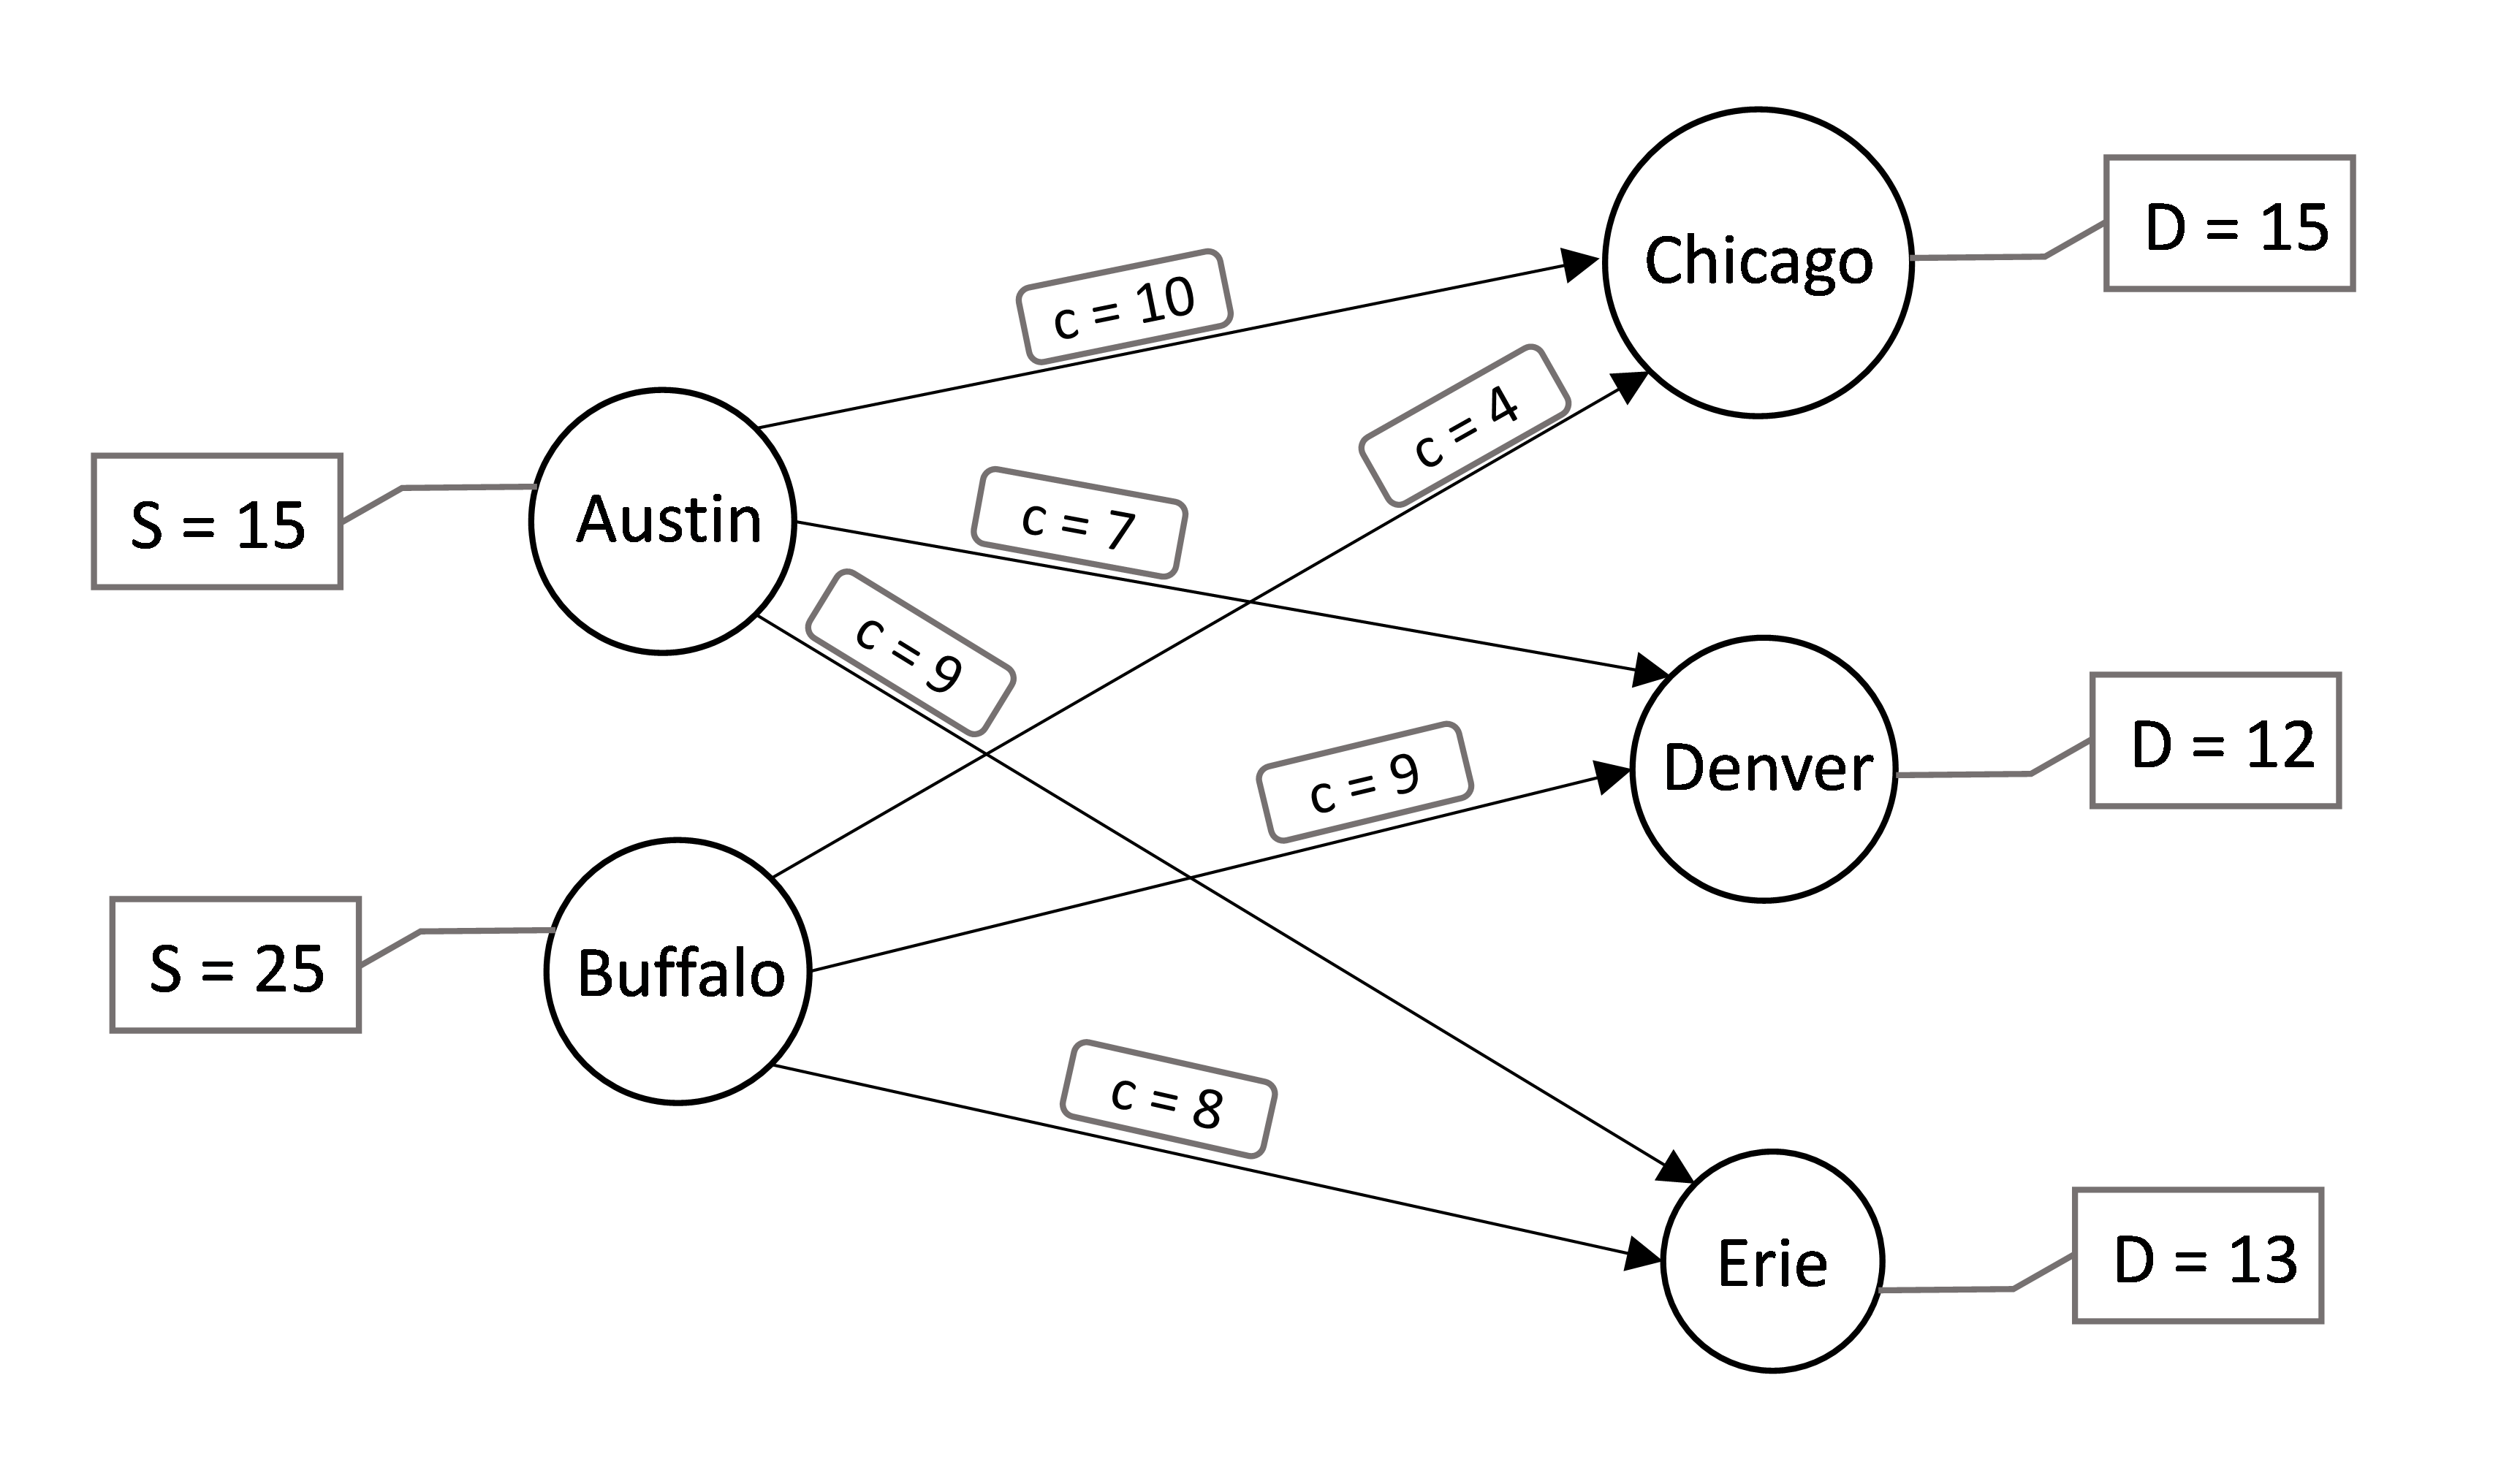
\includegraphics[scale=0.15]{part_1/chapter_1/figures/transp_ex1.png}
%\end{center}

\begin{figure}[h]
	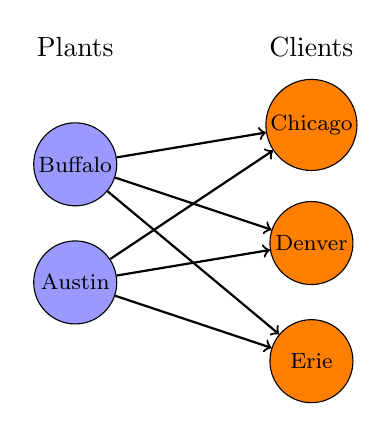
\begin{tikzpicture}[scale=1,
		node/.style={circle, fill=blue!40, draw, minimum size=3em, inner sep=1pt},
		node2/.style={circle, fill=orange, draw, minimum size=3em, inner sep=1pt}] 
    	\node[above] at (0, 4.75) {Plants};                                                                                  
    	\node[above] at (3, 4.75) {Clients};
	    \node[node] (1) at (0, 2) {\footnotesize Austin};
	    \node[node] (2) at (0, 3.5) {\footnotesize Buffalo};
	    \node[node2] (3) at (3, 4) {\footnotesize Chicago};
	    \node[node2] (4) at (3, 2.5) {\footnotesize Denver};
	    \node[node2] (5) at (3, 1) {\footnotesize Erie};
	    \foreach \x in {1,...,2} {
	       \foreach \y in {3,...,5} {
	          \draw[->, thick] (\x) -- (\y);
	          }}      
	\end{tikzpicture}
\end{figure}

\begin{table}[h]
	\begin{tabular}{r|ccc|c}
    	& & {\it Clients} &\\\hline
    	{\it Factory} & Chicago & Denver & Eire \\\hline
    	Buffalo 		  & 4       & 9      & 8    & 25 \\
    	Austin        & 10      & 7      & 9    & 600 \\\hline
    	Demands       & 15      & 12     & 13   & - \\\hline
	\end{tabular}
	\caption{Problem data: unit transportation costs, demands and capacities}
\end{table}

Solve the transportation problem to the minimum cost.
